\chapter{Autour d'un développement double-échelle}
\label{chap:two-scale}

Dans ce chapitre, on discute rapidement d'une démarche de développement double-échelle pour les problèmes à relaxation rapide de la forme
\begin{equation} \label{2s:pb:u}
    \pa_t u = -\frac{1}{\eps}Au + f(u), 
    \qquad
    u(0) = u_0 \in \setR^d
\end{equation}
avec $A$ un opérateur de relaxation et $u \mapsto f(u)$ un champ de vecteurs régulier. L'idée du développement double-échelle est d'écrire $t \mapsto u(t)$ comme une évaluation particulière d'une fonction à deux variables 
\begin{equation} \label{2s:eq:defU}
    u(t) = U(t,\tau)|_{\tau = t/\eps} .
\end{equation}
Cette approche a été un succès dans le contexte de problèmes hautement oscillants (voir~\cite{chartier.2015.uniformly, chartier.2020.derivative}), et est à la base des méthodes d'homogénéisation~\cite{allaire.1992.homogenization}. Dans ce contexte, on suppose que la nouvelle quantité $(t,\tau) \mapsto U(t,\tau)$ est périodique par rapport à la seconde variable $\tau$. 

Dans le cadre de problèmes à relaxation rapide, on suppose $\tau \in \setR_+$, et on injecte~\eqref{2s:eq:defU} dans~\eqref{2s:pb:u} pour obtenir le problème de transport pour $(t,\tau) \in [0,T] \times \setR_+$ 
\begin{equation} \label{2s:pb:trsp_U}
    \pa_t U + \frac{1}{\eps} \left(\pa_\tau + A \right) U
    = f(U) .
\end{equation}
De part la structure du problème, il faut définir une donnée initiale $\tau \mapsto U_I(\tau) := U(0,\tau)$ et une donnée au bord $t \mapsto U_B(t) := U(t,0)$, tel que sur le diagramme suivant: 

\usetikzlibrary{decorations.markings}
\begin{center}
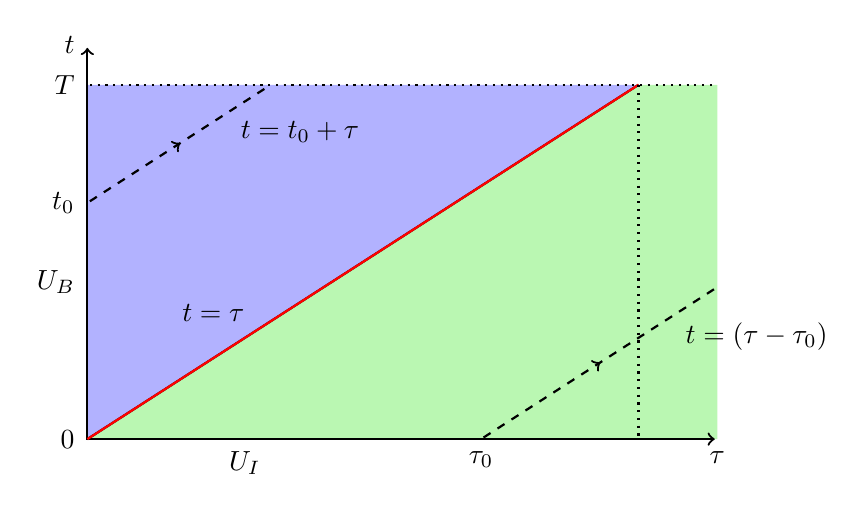
\begin{tikzpicture}
\begin{scope}[thick,decoration={
    markings,
    mark=at position 0.5 with {\arrow{>}}}
    ]
    \path[fill=blue,opacity=.3] (0,0) -- (7,4.5) -- (0,4.5);     
    \path[fill=green!80!olive,opacity=.3] (0,0) -- (7,4.5) -- (8,4.5) -- (8,0); 
    
    % Nodes
    \node[inner sep=0pt,label=left:{0}] (O) at (0,0) {};
    \node[inner sep=0pt,label=below:{$\tau$}] (tauf) at (8,0) {};
    \node[inner sep=0pt,label=below:{$\tau_0$}] (tau) at (5,0) {}; 
    \node[inner sep=0pt,label=left:{$t$}] (tf) at (0,5) {}; 
    \node[inner sep=0pt,label=left:{$T$}] (T) at (0,4.5) {}; 
    \node[inner sep=0pt,label=left:{$t_0$}] (t0) at (0,3) {};
    
    % Lines
    \draw[<->] (tf) -- (0,0) -- (tauf); 
    \draw[thick] (0,0) -- ++(7,4.5);
    \draw[thick,color=red] (0,0) -- ++(7,4.5);
    \draw[dotted] (T) -- ++(8,0); 
    \draw[dotted] (7,4.5) -- ++(0,-4.5); 
    \draw[dashed,postaction={decorate}] (t0) -- ++(2.33,1.5); 
    \draw[dashed,postaction={decorate}] (tau) -- ++(3,1.93); 
    
    % Text
    \node at (1.6,1.6) {$t=\eps\tau$};
    \node at (2.7,3.9) {$t=t_0 + \eps\tau$};
    \node at (8.5,1.3) {$t=\eps(\tau-\tau_0)$};
    % \node at (2,2.8) {$\mathbb{U}_T\eeps$};  
    % \node at (4.5,1.3) {$\mathbb{L}_T\eeps$}; 

    % Conditions
    \node at (-.4,2) {$U_B$};
    \node at (2,-.3) {$U_I$};
\end{scope}
\end{tikzpicture}
\end{center}

\noindent
Les valeurs qui nous intéressent sont sur la ligne caractéristique $t = \eps\tau$, en rouge. La donnée initiale $U_I$ permet de déterminer les valeurs de $U$ dans le domaine vert sous cette caractéristique, tandis que la donnée au bord $U_B$ détermine les valeurs dans le domaine bleu au-dessus de la caractéristique. 


\paragraph{Caractère bien posé du problème \\}
Discutons d'abord du caractère bien posé d'un problème de la forme~\eqref{2s:pb:trsp_U}. Le caractère bien posé de ce problème se fait naturellement le long des caractéristiques, qui s'écrivent $t = t_0 + \eps\tau$ au-dessus de la diagonale $t = \eps\tau$, et $t = \eps(\tau - \tau_0)$ en-dessous, avec $(t_0,\tau_0) \in [0,T] \times \setR_+$. Ainsi, si les données $U_I$ et $U_B$ sont bornées, quitte à réduire le temps d'existence $T$, le problème est bien posé. Cependant, avec cette approche, on ne précise pas la régularité de la solution obtenue, le problème est bien posé dans $L^{\infty}([0,T] \times \setR_+)$. Si en outre $U_B$ et $U_I$ sont continues avec $U_B(0) = U_I(0) = u_0$, le problème est bien posé dans $C^0([0,T] \times \setR_+)$. 

Si on veut que le problème soit bien posé dans $C^1$, il faut que $U_B$ et $U_I$ soient continues, mais aussi qu'à la limite $t \rightarrow 0$ et $\tau \rightarrow 0$, ces données soient compatibles. En effet, dans~\eqref{2s:pb:trsp_U}, on a en $(t,\tau) = (0,0)$, 
\begin{equation*}
    \pa_t U_B(0) + \frac{1}{\eps}(\pa_\tau + A)U_I(0) = f(u_0) .
\end{equation*}
Si cette condition est respectée, on remarque que la dérivée $V = \pa_t U$ vérifie le problème de transport 
\begin{equation*}
    \pa_t V + \frac{1}{\eps}(\pa_\tau + A) V = f'(U)V .
\end{equation*}
Les conditions initiales et au bord associé à ce problème sont continues, donc cette dérivée est continue. Le même raisonnement peut être tenu pour $\pa_\tau U$, si bien que la fonction $(t,\tau) \mapsto U(t,\tau)$ est de classe~$C^1$. À l'ordre~2, on trouve
\begin{equation*}
    \pa_t^{\: 2} U_B(0) - \frac{1}{\eps^2}(\pa_\tau + A)^2 U_I(0)
    = f'(u_0)\pa_t U_B(0) 
        - \frac{1}{\eps}(\pa_\tau + A) f(U_B(\tau))|_{\tau = 0} ,
\end{equation*}
et on peut dériver des conditions similaires aux ordres supérieurs. Si les données initiale et au bord sont de régularité $C^n$ avec des dérivées bornées à tout ordre (jusqu'à $n$), et que les conditions de compatibilité sont respectées jusqu'à l'ordre $n$, alors, quitte à modifier le temps $T$ d'existence de la solution, le problème~\eqref{2s:pb:trsp_U} est bien posé dans~$C^n([0,T] \times \setR_+)$.

\paragraph{Motivation et calcul numérique\\}

Évidemment, on ne peut pas résoudre le problème directement le long d'une caractéristique, puisque cela revient à résoudre un problème de la forme~\eqref{2s:pb:u}. En revanche, on peut choisir la donnée initiale et la donnée au bord de sorte que le problème soit bien posé au sens où un certain nombre de dérivées $\pa_t U$ soient uniformément bornées. Par exemple en choisissant 
\begin{equation*}
    U(0,\tau) = e^{-\tau A} u_0 ,
\end{equation*}
on a $\pa_t U (0,\tau) = f(e^{-\tau A} u_0)$. Cependant à l'ordre supérieur on peut calculer 
\begin{equation*}
    \pa_t^{\:2}U(0,\tau) = \pa_u f(e^{-\tau A}u_0)f(e^{-\tau A}u_0) + \frac{1}{\eps} [f,A](e^{-\tau A} u_0) 
\end{equation*}
avec $[f,A] = \pa_u f \cdot A - A f$. En supposant que $A$ et $f$ ne commutent pas (sinon on pourrait simplement faire du splitting sur le problème d'origine), cette donnée est raide, et quelle que soit la donnée au bord qu'on choisira, le problème ne sera pas uniformément (i.e. indépendamment de $\eps$) bien posé dans $C^2([0,T] \times \setR_+)$. 

Supposons maintenant que l'on dispose d'une donnée initiale $\tau \mapsto U_I(\tau)$ et d'une donnée au bord $t \mapsto U_B(t)$ compatibles à l'ordre~2 et telles que ces données et leurs dérivées jusqu'à l'ordre~2 soient uniformément bornées. Alors en supposant qu'on connait de manière exacte\footnote{%
    Si le comportement selon $\tau$ n'est pas connu parfaitement, le problème devient plus complexe à résoudre car il faut discrétiser l'espace de cette variable, et les schémas numériques doivent prendre cette discrétisation en compte dans la donnée au bord. Voir par exemple~\cite{boutin.2019.high}.
} le comportement par rapport à $\tau$ d'une approximation de la solution à un temps $t_n$, $U_n(\tau) \approx U(t_n, \tau)$, alors on peut calculer la solution au temps $t_{n+1} = t_n + \Dt$ avec la formule
\begin{equation*}
    \frac{U_{n+1}(\tau) - U_n(\tau)}{\Dt} 
        + \frac{1}{\eps}(\pa_\tau + A) U_{n+1}(\tau)
    = f(U_n(\tau)) ,
\end{equation*}
soit de manière explicite en posant $\mu = \eps/\Dt$, 
\begin{equation*}
    U_{n+1}(\tau) = e^{-\tau (\mu I + A)} U_B(t_{n+1}) 
        + \mu \int_0^{\tau} e^{(\sigma - \tau)(\mu I + A)} \left(
            U_n(\sigma) + \Dt\: f\big( U_n(\sigma) \big)
        \right) \D\sigma .
\end{equation*}
En s'inspirant des preuves de~\cite{chartier.2015.uniformly}, on peut alors prouver que si la dérivée seconde $\pa_t^{\: 2} U$ peut être bornée indépendamment de~$\eps$, alors il existe $C$ et $\Dt_0$ indépendants de $\eps$, tels que pour toute discrétisation $(t_n)_{0 \leq n \leq N}$ de pas de temps $\Dt < \Dt_0$, l'erreur du schéma prend la forme
\begin{equation*}
    \sup_{\tau \in \setR_+} | U_{n} - U(t_n, \cdot) |
    \leq C \Dt \sup_{(t,\tau) \in [0,T] \times \setR_+} 
        | \pa_t^{\: 2} U(t,\tau) | 
\end{equation*}
pour tout $0 \leq n \leq N$.

De la même manière, si le problème est uniformément bien posé dans $C^3$, on peut construire un schéma à deux étages d'ordre~2, comme cela a pu être proposé dans un cadre hautement oscillant chez~\cite{chartier.2015.uniformly}. On peut certainement construire des schémas d'ordre plus élevé en s'inspirant des méthodes de type Adams-Bashforth utilisées dans~\cite{chartier.2020.derivative}. Néanmoins, il faut pour cela être capable de construire des données initiale et au bord pour que le problème soit uniformément bien posé dans $C^2,\ C^3$ ou dans un espace encore plus régulier. 


\paragraph{Choix de la donnée initiale\\}
Un moyen de trouver un problème uniformément bien posé est d'écrire $U(t,\tau)$ comme une série en puissances de~$\eps$, 
\begin{equation*}
    U(t,\tau) = \sum_{n \geq 0} \eps^n U_n (t,\tau) .
\end{equation*}
On effectue ensuite une séparation d'échelles afin de trouver, pour les premiers termes, 
\begin{equation*}
    \left\{\begin{array}{ll}
        \pa_\tau U_0 + A U_0 = 0 & (\eps^{-1}) \\
        \pa_\tau U_1 + AU_1 = f(U_0) - \pa_t U_0 
        & (\eps^0) \\
        \pa_\tau U_2 + AU_2 = f'(U_0)U_1 - \pa_t U_1
        \qquad
        & (\eps^1) \\
        \quad\vdots
    \end{array}\right.
\end{equation*}
Ainsi on retrouve le premier terme,
\begin{equation*}
    U_0(t,\tau) = e^{-\tau A} \widetilde{u}_0(t)
\end{equation*}
et si on néglige les termes d'ordre $\eps$ et au-delà dans la série, on peut choisir $t \mapsto u_0(t)$ librement. Si on cherche à étendre le développement, en revanche, on trouve 
\begin{equation*}
    U_1(t,\tau) = e^{-\tau A} \widetilde{u}_1(t)
    + \int_0^{\tau} e^{(\sigma-\tau)A} \left(
        f(e^{-\tau A}\widetilde{u}_0(t)) - e^{-\tau A} \pa_t \widetilde{u}_0(t) 
    \right) \D \sigma .
\end{equation*}
Si on veut que cette quantité soit sous forme d'une série exponentielle (cette forme serait avantageuse pour l'implémentation, car on peut alors discrétiser $\tau$ de manière adaptée), il faut choisir $\pa_t \widetilde{u}_0$ comme étant la composante en $e^{-\tau A}$ de $f(e^{-\tau A}\widetilde{u}_0)$. La même chose se produit à l'ordre suivant, où~$\pa_t \widetilde{u}_1$ est déterminé comme étant la composante en~$e^{-\tau A}$ de~$f'(U_0)U_1$, etc. Les valeurs initiales~$\widetilde{u}_k(0)$ sont encore libres.

Enfin, on peut tronquer la série afin de choisir une donnée initiale 
\begin{equation*}
    U_I\rk n(\tau) = \sum_{k=0}^n \eps^k U_n(0,\tau) .
\end{equation*}
Il faut ensuite déterminer les données initiales~$\widetilde{u}_k(0)$ de sorte à obtenir un problème bien posé dans $C^{n+1}([0,T] \times \setR_+)$, et résoudre les problèmes associés à chacune de ces variables pour obtenir une donnée au bord 
\begin{equation*}
    U_B(t) = \sum_{k = 0}^n \eps^k \widetilde{u}_k(t) .
\end{equation*}
Nous n'avons cependant pas de méthode pour trouver ces données au bord, et nous n'avons pas non plus étudié les conséquences d'avoir des données compatibles \enquote{à~$\eps^{n}$ près.}

\begin{FRremark}
    On serait tenté de penser que la définition de $U_B(t)$ a peu d'importance tant que les conditions de compatibilité sont vérifiées. Cependant, cette définition est certainement cruciale pour pouvoir implémenter la méthode. En effet, en ne considérant que les conditions de compatibilité, on pourrait définir pour un problème dans $C^2([0,T] \times \setR_+)$
    \begin{equation*}
        U_B(t) = u_0 + t\ \pa_t U_B(0) 
            + \frac{t^2}{2} \pa_t ^{\:2} U_B(0) ,
    \end{equation*}
    mais alors à un temps $t > 0$ fixé, on observe que la solution $\tau \mapsto U(t,\tau)$ comporte deux parties de comportement distinct de part et d'autre de $t/\eps$. La partie de gauche ressemble à une parabole, de la forme $\alpha (\eps\tau)^2 + \beta\eps\tau + \gamma$, tandis que la partie de droite est exponentielle. La discrétisation de la variable $\tau$ doit alors capturer ces deux comportements, tandis qu'un choix judicieux de $U_B(t)$ permet de conserver une forme exponentielle pour tout $(t,\tau)$. 
\end{FRremark}

On retrouve ainsi formellement la même construction que dans le Chapitre~\ref{chap:dissip-mima}. La donnée initiale $U_I$ peut en effet s'écrire  
\begin{equation*}
    U_I(\tau) = \Omega^\eps_\tau \circ \big( \Omega^\eps _0 \big)^{-1} .
\end{equation*}
Ce lien entre décomposition micro-macro et décomposition double-échelle est également soulevé dans le cadre périodique chez~\cite{chartier.2020.derivative}. La nouveauté par rapport à ce cadre est la donnée au bord $t \mapsto U_B(t)$, et on a vu que la bonne détermination de cette donnée est problématique. Tracer un lien entre cette donnée au bord et la construction micro-macro donnerait certainement des pistes pour déterminer les valeurs initiales $\widetilde{u}_k(0)$ associées au problèmes au bord. 